\section{Experiments}
\label{sec:experiments} 

In our experiments, we test \ModelAcronym{} with two VLA backbones: $\pi_0$~\citep{black2024pi_0} and OpenVLA~\citep{kim2024openvla}. We compare \ModelAcronym{} to alternative action tokenization schemes and ablate key design decisions. We then compare $\pi_0$ models trained with \ModelAcronym{} tokenization to the state-of-the-art $\pi_0$ flow-matching (diffusion) VLA, and test the scaling of autoregressive VLA training with \ModelAcronym{} to large, cross-embodied datasets with 10k hours of dexterous robot manipulation data.


\subsection{Experimental Setup}
\label{sec:exp_setup}

\noindent\textbf{Policy implementation.}
We test different tokenization schemes for autoregressive VLA training with popular VLA backbones. For most of our experiments, we use $\pi_0$~\citep{black2024pi_0}, a VLA based on PaliGemma-3B~\citep{beyer2024paligemma}. We also test with OpenVLA~\citep{kim2024openvla}, which is built on Prismatic~7B~\citep{karamcheti2024prismatic}. During training, we tokenize 1-second action chunks and overwrite the least used tokens in the VLM vocabulary with the resulting action tokens, following prior VLAs~\citep{rt22023arxiv,kim2024openvla}. We fine-tune the VLA models for robot action prediction, without weight freezing. %
We provide more details on the policy training setup in \cref{sec:app_policy_training_details}.

\begin{figure}[t]
    \centering
    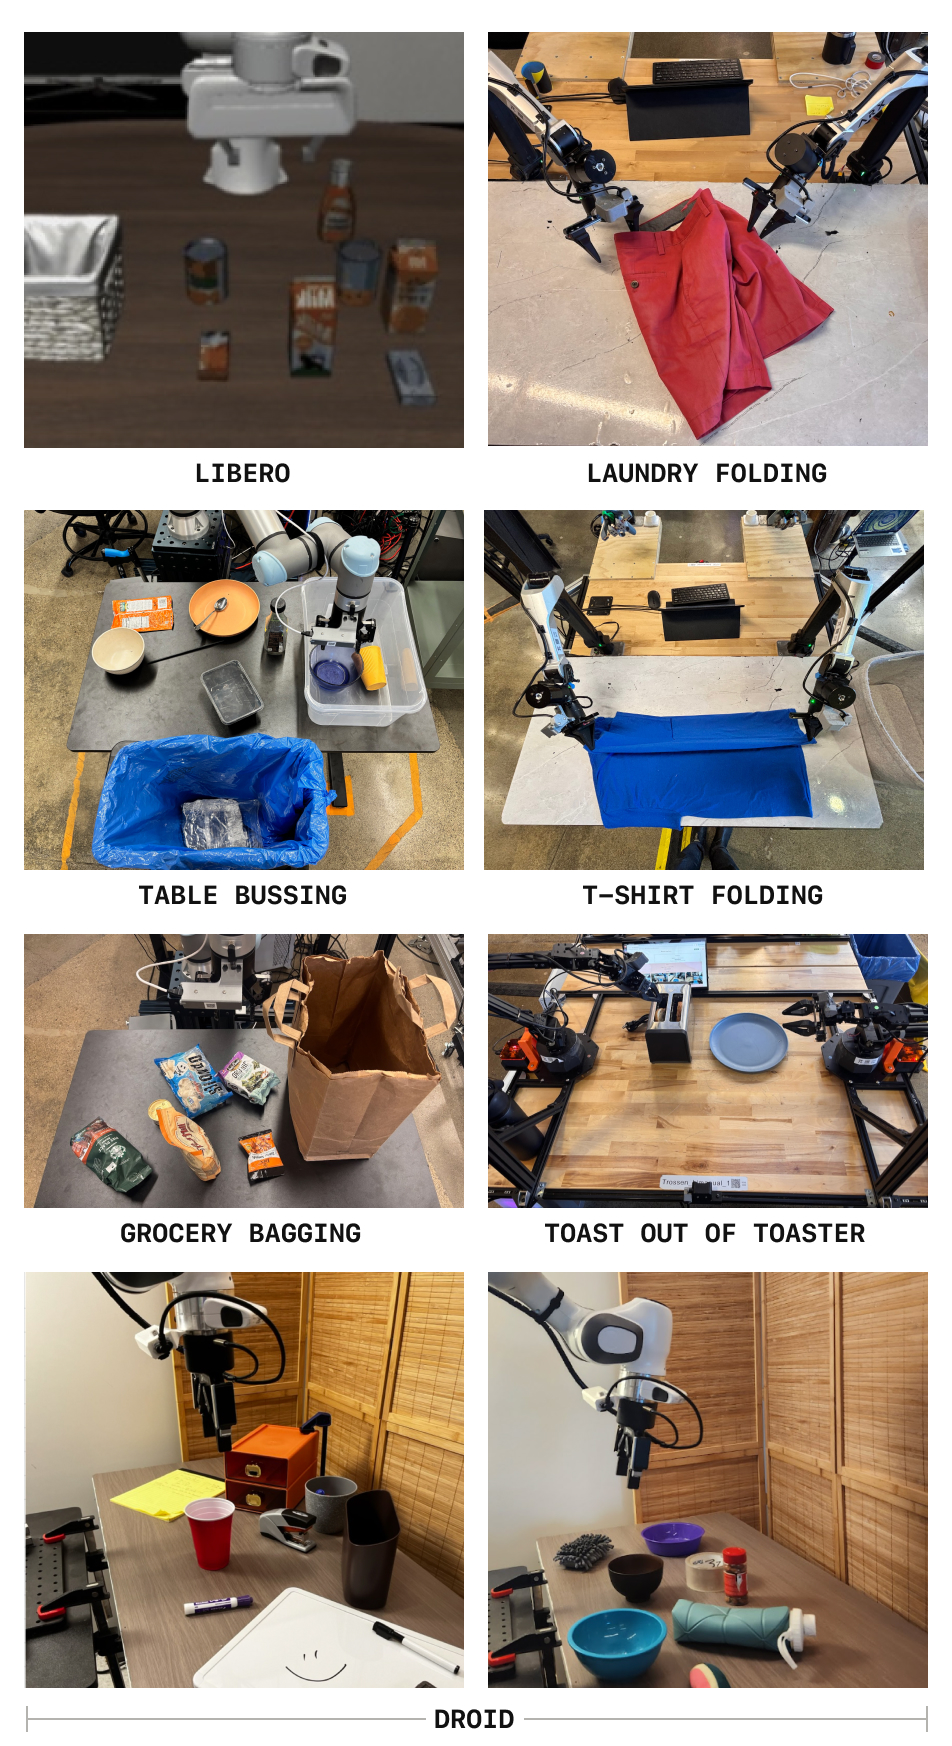
\includegraphics[width=0.9\linewidth]{figures/environments.jpg}
    \caption{\textbf{Evaluation environments.} We test \ModelAcronym{} across 7~evaluation environments: 6~real-robot tasks and 1~simulation environment. The tasks are designed to test VLA performance on highly dexterous tasks, like folding cloths from a laundry basket (``Laundry Folding''), and generalization, e.g., zero-shot table-top manipulation in unseen environments (``DROID'').
    }
    \label{fig:environments}
\end{figure}

\noindent\textbf{Evaluation tasks.}
We develop a suite of 7~evaluation tasks (6~real robot, 1~simulated; see \cref{fig:environments}), designed to test VLA performance on both, highly dexterous tasks like laundry folding, and generalization tasks, like performing table-top manipulations 0-shot in unseen environments.
\begin{itemize}
    \item \textbf{Libero}: We test on the Libero~\citep{liu2024libero} simulated benchmark suites. We measure average performance across Libero-Spatial, Libero-Object, Libero-Goal, and Libero-10. 
    \item\textbf{Table bussing}~\citep{black2024pi_0} (20~Hz): a UR5 single-arm robot needs to clean a table, sorting 12~objects into a trash bin (for trash) and a plastic container (for plates, bowls, cups and cutlery). The task requires precise grasping of various objects.
    \item\textbf{T-Shirt folding}~\citep{black2024pi_0} (50~Hz): a bi-manual ARX robot setup needs to fold various shirts on a stationary table top. At the beginning of the task, the shirts are placed flat on the table. Succeeding at the task requires precise grasps and movements to fold the shirt.
    \item\textbf{Grocery bagging}~\citep{black2024pi_0} (20~Hz): a UR5 single-arm robot needs to pack seven objects from a table into a grocery bag, taking care to not topple or rip the bag in the process. This task requires picking a diverse set of objects and carefully inserting them into the bag.
    \item\textbf{Toast out of toaster}~\citep{black2024pi_0} (50~Hz): a bimanual Trossen Viper-X robot needs to remove two slices of bread from a toaster and place them on a plate. This task requires precise grasping and placement of the bread slices.
    \item\textbf{Laundry folding}~\citep{black2024pi_0} (50~Hz): a bi-manual ARX robot needs to take shirts and shorts from a basket, flatten them on a table, fold and stack them. This is the most dexterous task we test. It requires precise grasps, dynamic motions to flatten the cloths, retrying and corrections when cloths got tangled up, and precise placements of the folded cloths on the existing stack of cloths. We report success rate on individual clothing items.
    \item\textbf{Zero-shot DROID tabletop manipulation}~\citep{khazatsky2024droid} (15~Hz): we test a policy trained on the full DROID dataset across various table-top manipulation tasks like picking and placing objects, wiping, opening and closing drawers etc. Importantly, we test the policy in a completely \emph{unseen} environment, with a new table setup, background, novel objects, viewpoint and table height. To our knowledge, this is the first ``zero-shot'' evaluation of DROID policies in a completely unseen environment, without co-training or fine-tuning, simply by prompting a pre-trained model with natural language.
\end{itemize}
Following \citet{black2024pi_0}, we use grocery bagging, the toaster task, and laundry folding only to evaluate our most powerful, generalist VLA in \cref{sec:generalist_vlas}. We provide additional details on training datasets and evaluation tasks in \cref{sec:app_exp_task_details}.

\noindent\textbf{Comparisons.}
We test \textbf{\ModelAcronym}, our DCT-based action tokenization approach, trained on each evaluation dataset individually, and \textbf{\ModelUniversalAcronym}, our universal DCT-based action tokenizer, trained on a large dataset of 1M~action sequences. Note that we trained the universal tokenizer on the most diverse real robot dataset we could assemble, which includes data from our real-robot evaluation tasks. We compare both tokenizers to the per-dimension binning scheme used by prior autoregressive VLAs like RT-2~\citep{rt22023arxiv}, RT-2-X~\citep{open_x_embodiment_rt_x_2023} and OpenVLA~\citep{kim2024openvla}, dubbed \textbf{na\"{i}ve tokenization}. We apply the binning tokenization to each time step in the action chunk separately and then concatenate. Finally, while our approach provides a compressed tokenization without the need to train any separate model, we can consider an alternative compression scheme that instead trains a model to produce a quantized representation of the action chunk via \textbf{FSQ}~\cite{fsq}, a simpler alternative to VQ-VAE~\cite{vqvae}. This tokenization strategy has been previously used to tokenize high-dimensional image data~\citep{fsq,yu2023magvit}, and can be viewed as an ablation of our compression-based approach, utilizing compressed representations but with a more complex learning-based alternative to our relatively simple DCT-based method.

\subsection{Comparing Action Tokenizers for VLA Training}
\label{sec:main_comparison}

\begin{table}[h]
\centering
\begin{tabular}{l|c|c|c|c|c}
\toprule
\multirow{2}{*}{Dataset} & \multirow{2}{*}{\begin{tabular}[c]{@{}c@{}}Action\\ Dimension\end{tabular}} & \multirow{2}{*}{\begin{tabular}[c]{@{}c@{}}Control\\ Frequency\end{tabular}} & \multicolumn{2}{c|}{Avg. Token} & \multirow{2}{*}{Compression} \\
 &  &  & Naive & \ModelAcronym &  \\
\midrule
BridgeV2 & 7 & 5\;Hz & 35 & \cellcolor{lightgreen}20 & 1.75 \\
DROID & 7 & 15\;Hz & 105 & \cellcolor{lightgreen}29 & 3.6\\
Bussing & 7 & 20\;Hz & 140 & \cellcolor{lightgreen}28 & 5.0\\
Shirt Fold & 14 & 50\;Hz & 700 & \cellcolor{lightgreen}53 & 13.2\\
\bottomrule
\end{tabular}
\caption{\textbf{Comparison of the average token count per action chunk} for na\"{i}ve tokenization and \ModelAcronym. We use 1-second chunks in all datasets. With our method, each chunk requires many fewer tokens, particularly for high-frequency domains such as the T-shirt folding task, indicating that it is more effective at removing redundancy.}
\label{tab:compression_ratios}
\end{table}

We first provide a comparison of compression rates between our proposed \ModelAcronym~tokenizer and the na\"{i}ve binning scheme used in prior works in \cref{tab:compression_ratios}. We use 1-second action chunks from datasets with various action dimensionalities and control frequencies. For both approaches we use the default hyperparameters, which have comparable tokenization errors. We see that \ModelAcronym~achieves a significant compression of the input action sequences across all datasets. The compression benefits are especially pronounced for datasets with high-frequency action data. Interestingly, \ModelAcronym~consistently generates roughly 30 action tokens per chunk per robot arm (i.e., 60 tokens for the bi-manual setup) in each of the domains. This suggests that \ModelAcronym~finds a representation that approximates the complexity of the underlying action signal, and is largely independent of the frequency of the action data.

We note that this compression is not entirely lossless, with a trade-off between compression ratio and reconstruction accuracy determined by the scale parameter $\gamma$ from \cref{alg:fast}. Figures in \cref{tab:compression_ratios} are at comparable reconstruction accuracy. Please see \cref{sec:app_compression_plots} for plots showing the trade-off between compression and fidelity for each of the tokenizers we compare. 






\begin{figure*}[t]
    \centering
    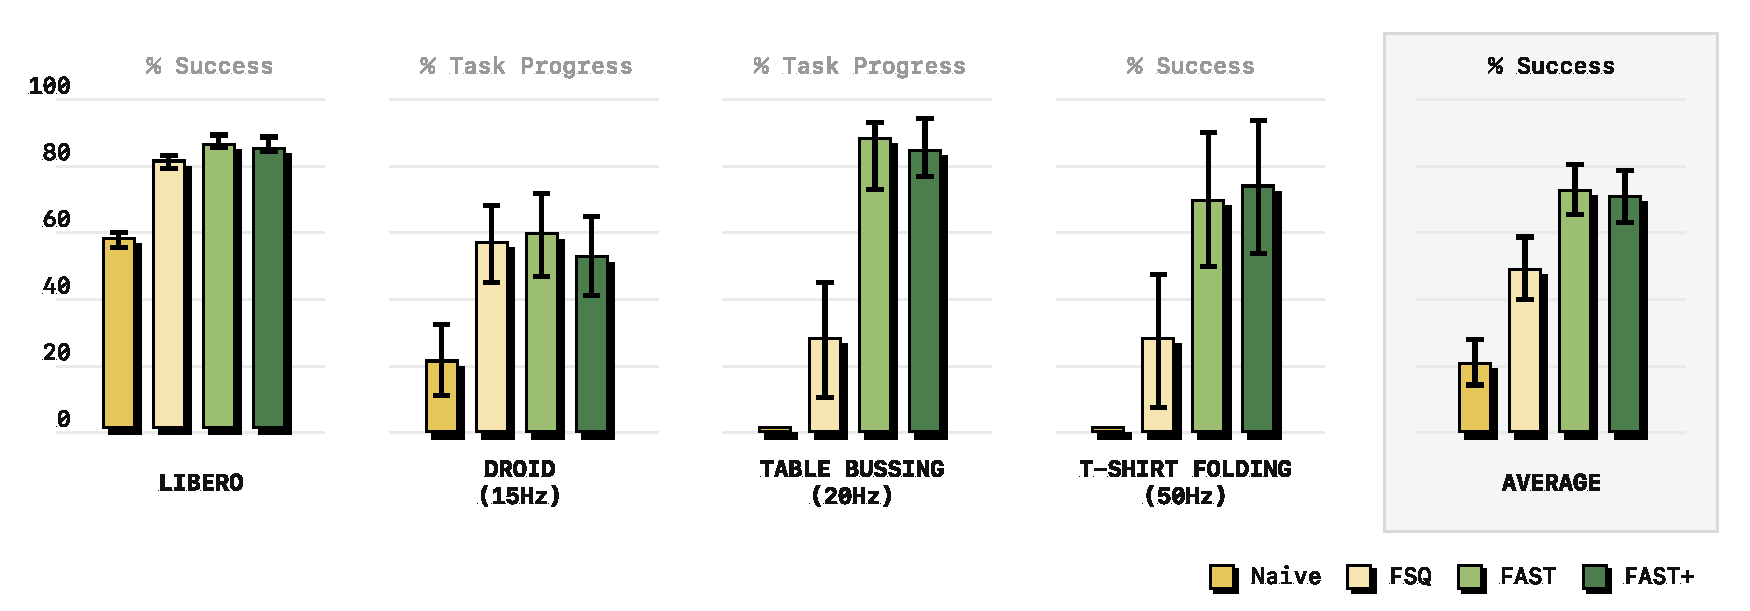
\includegraphics[width=0.8\linewidth]{figures/main_result.pdf}
    \caption{\textbf{Comparison of policy performance using different tokenization approaches.} We find that tokenization approaches that compress action targets (\ModelAcronym, FSQ) lead to substantially more efficient training than the na\"{i}ve binning tokenization used in prior VLAs. Overall, we find that \ModelAcronym~leads to more effective policy training than FSQ, particularly on dexterous real-robot tasks. Our universal tokenizer, \ModelUniversalAcronym, matches the performance of dataset-specific tokenizers. We report mean and 95\% CI.
    }
    \label{fig:tokenization_comparison}
\end{figure*}

Next, we train policies using the policy architecture and tokenization approaches described in \cref{sec:exp_setup}.
We report results in \cref{fig:tokenization_comparison}.

Overall, we find that the na\"{i}ve tokenization applied in prior works struggles to learn effective policies on high-frequency robot data. This is particularly apparent for the highest frequency tasks in our evaluations: Table Bussing (20Hz) and T-Shirt Folding (50Hz). On both tasks, policies trained with na\"{i}ve tokenization are unable to make progress on the task. 

In contrast, we find that compression-based tokenization leads to effective training. Comparing \ModelAcronym{} to our FSQ baseline, we find that \ModelAcronym{} is as good or at times better, particularly on the dexterous, high-frequency tasks, despite being much simpler and requiring no separate neural network training. %

\begin{figure}[t]
    \centering
    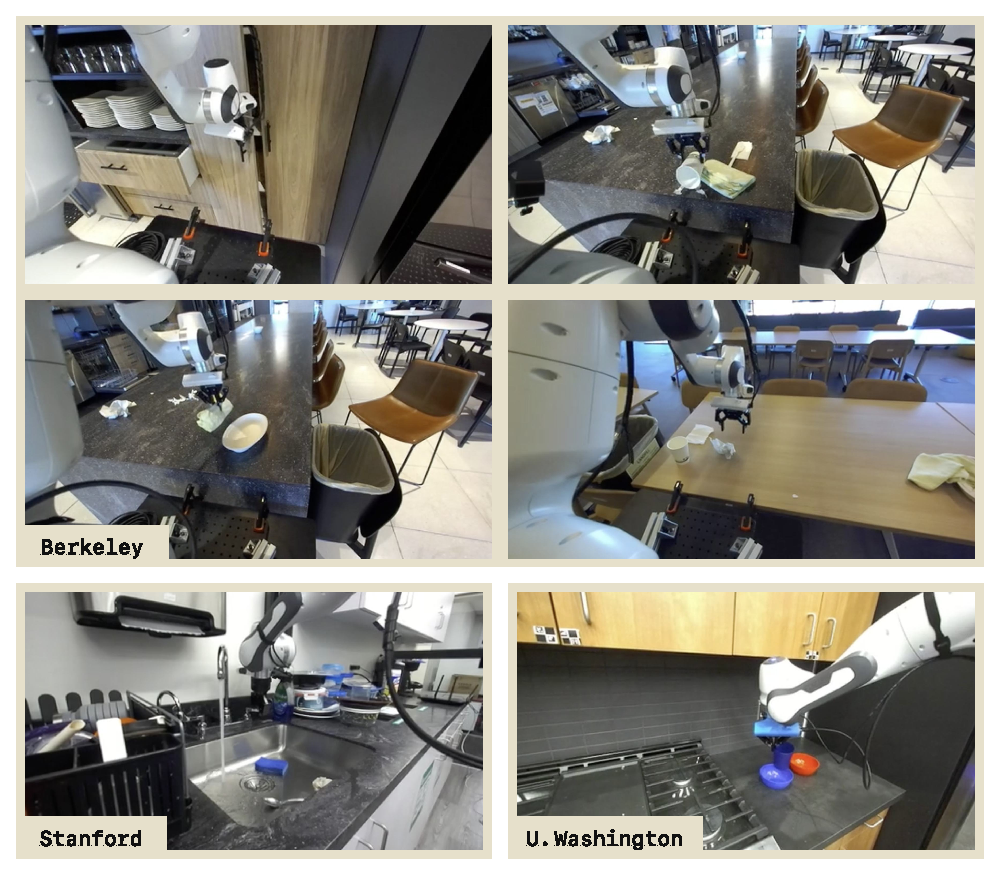
\includegraphics[width=\linewidth]{figures/droid_quali.pdf}
    \caption{\textbf{Evaluation environments of \ModelAcronym{} policy trained on DROID~\citep{khazatsky2024droid}.} We find that the same policy checkpoint generalizes robustly, and performs various simple table-top tasks \emph{zero-shot} across three university campuses. 
    }
    \label{fig:droid_quali}
\end{figure}

Notably, \ModelAcronym{} tokenization enables the first successful training of a strong generalist policy on the DROID dataset~\citep{khazatsky2024droid}, which can be evaluated \emph{zero-shot} in unseen environments, without fine-tuning, by simply prompting it in natural language. All prior works, including the original DROID paper~\citep{khazatsky2024droid} and OpenVLA~\citep{kim2024openvla}, did not show zero-shot results and focused entirely on co-training or fine-tuning evaluations instead. We demonstrate the generality of our DROID policy by testing it on various table-top manipulation tasks in environments across three university campuses (\cref{fig:droid_quali}).
Out of the box, the policy can competently perform simple manipulation tasks, like picking and placing objects, opening and closing cupboards and turning on faucets, across a wide range of scenes and camera viewpoints. Even unsuccessful trials show sensible behavior, like approaching the handles of microwave and dish washer doors, even if ultimately failing to open them. We show success and failure videos on our website. While far from perfect, the level of generality and robustness of this policy substantially exceeds that of prior DROID policies. %


\subsection{Universal Action Tokenizer}
\label{sec:uniact}

\begin{figure}[t]
    \centering
    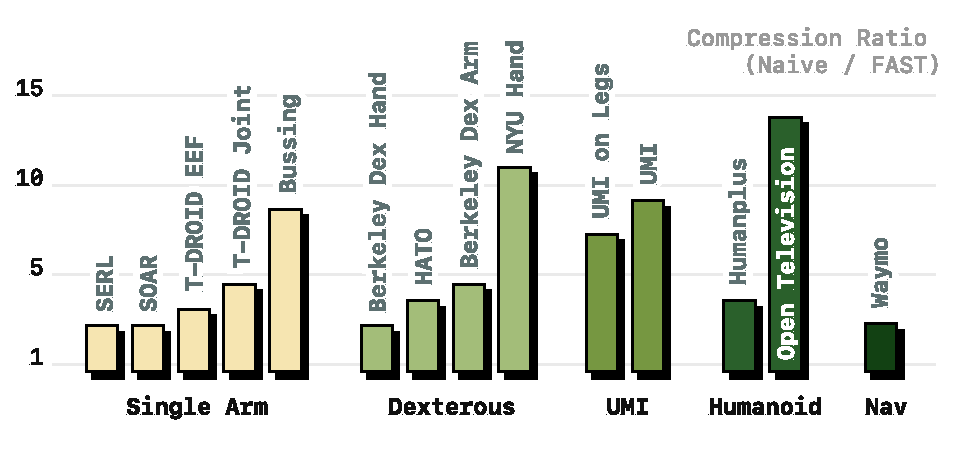
\includegraphics[width=\linewidth]{figures/bench_test_compression.pdf}
    \caption{\textbf{Universal tokenizer.} We test the compression rate achieved by our {\ModelUniversalAcronym} tokenizer vs. na\"{i}ve tokenization across diverse robot datasets, \emph{unseen} during tokenizer training. We find that {\ModelAcronym} is effective across a wide range of robot morphologies, action spaces and control frequencies.
    }
    \label{fig:universal_tokenizer_results}
\end{figure}

In this section, we evaluate the performance of our \emph{universal} action tokenizer, \ModelUniversalAcronym, which we trained on 1M real robot action sequences (see \cref{sec:universal_tokenizer}). 
To test the \emph{generality} of the tokenizer, we assemble a diverse set of small testing datasets. This set spans a wide range of robot morphologies, action spaces, and control frequencies (see \cref{fig:universal_tokenizer_results}, with a full list of datasets in \cref{sec:app_univeral_test_set}). Note that none of these datasets is part of the tokenizer training set. They thus test a scenario in which the tokenizer is applied to a completely new robot setup without recomputing the tokenization. We find that the \ModelUniversalAcronym{} tokenizer achieves good compression performance across a wide range of robot datasets, reducing the number of action tokens by 2x across all datasets, and significantly more on some.

We also test performance of the universal tokenizer for policy training, and report results alongside the per-dataset tokenizers in \cref{fig:tokenization_comparison}. 
Across all tasks, the \emph{universal} tokenizer closely matches the performance of the dataset-specific \ModelAcronym~tokenizers, suggesting that the universal tokenizer can be used as a strong default for robot action tokenization.


\subsection{Ablation Studies}

We analyze two key aspects of our method:
(1)~Is our \ModelAcronym~tokenization approach \emph{independent} of the underlying VLA backbone? (2)~How important is the BPE compression step, the only learned component of our tokenization pipeline.

\begin{wrapfigure}{r}{0.4\linewidth}
    \centering
    \vspace{-0.3cm}
    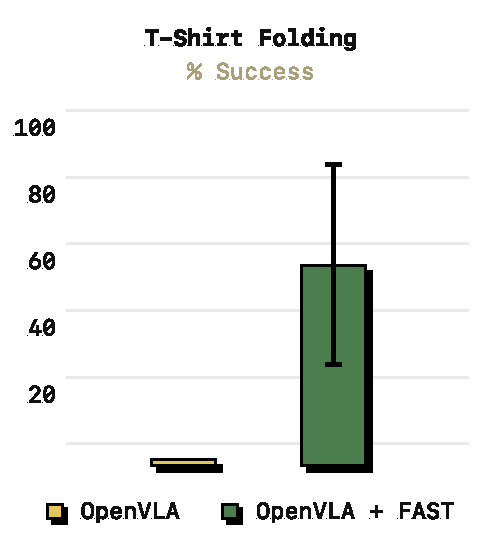
\includegraphics[width=\linewidth]{figures/openvla_results.pdf}
    \label{fig:openvla_results}
    \vspace{-0.3cm}
\end{wrapfigure}
To answer the first question, we train an OpenVLA policy~\citep{kim2024openvla} on the challenging high-frequency T-shirt folding dataset, comparing the na\"{i}ve tokenization approach originally used in OpenVLA to our \ModelUniversalAcronym{} tokenizer. To comply with the task setup, we modify the OpenVLA model code to accept multiple input images and predict 1-second action chunks. The results on the right demonstrate that \ModelAcronym{} is able to significantly boost performance of OpenVLA, enabling it to train effectively on high-frequency robot manipulation data. This suggests, that our tokenization approach is \emph{independent} of the underlying model backbone, and may be easily applied to a wide range of pre-trained autoregressive transformer models.

\begin{wrapfigure}{r}{0.4\linewidth}
    \centering
    \vspace{-0.3cm}
    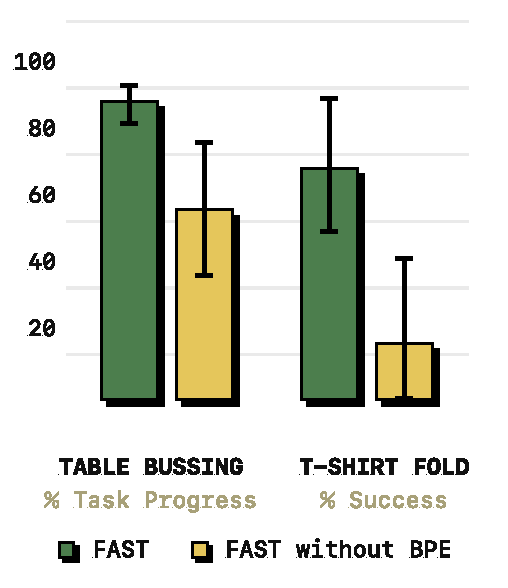
\includegraphics[width=\linewidth]{figures/nobpe_results.pdf}
    \label{fig:openvla_results}
    \vspace{-0.3cm}
\end{wrapfigure}
Secondly, we ablate the BPE encoding step on the table bussing and T-shirt folding tasks. The figure on the right shows that the resulting policies \emph{without BPE encoding} achieve worse rollout performance (but still outperform na\"{i}ve tokenization). Intuitively, the DCT transform still concentrates most of the signal's information in a few tokens, improving the learning signal. However, without BPE, there is a large number of repeated 0-tokens which dilute the learning signal and also significantly slow down inference, since models need to autoregressively predict hundreds of action tokens, ultimately leading to worse policy performance.


\subsection{Comparing \ModelAcronym{} to Diffusion}
\label{sec:ar_vs_diffusion}


In this section, we compare $\pi_0$, a state-of-the-art diffusion VLA, to our model that combines $\pi_0$ with \ModelAcronym{} and uses autoregressive decoding. We compare the performance of both models on the tasks from \cref{sec:main_comparison}. %

\begin{figure}[t]
    \centering
    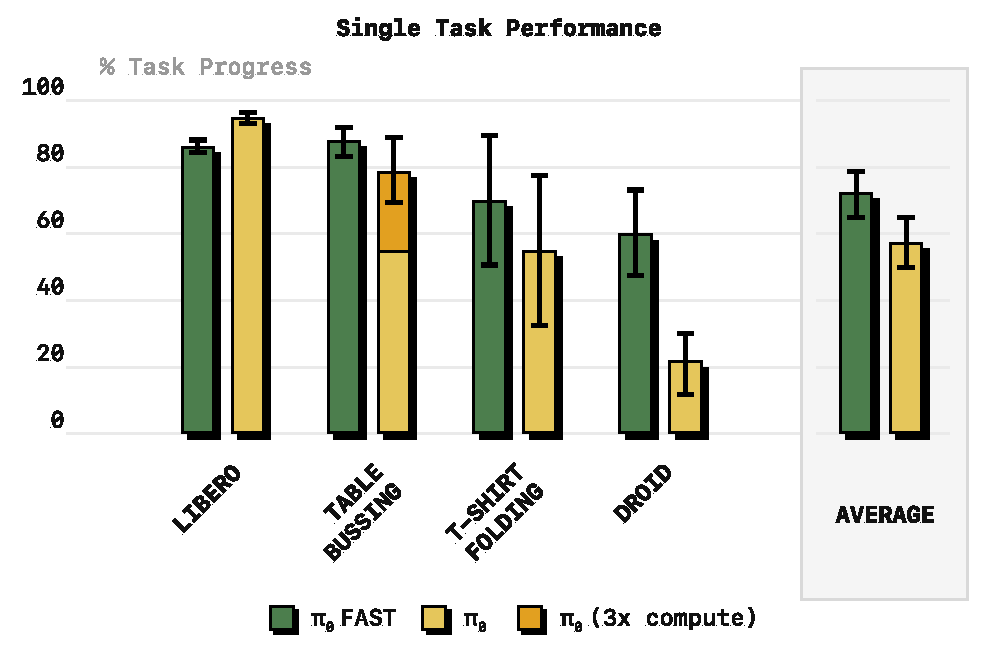
\includegraphics[width=\linewidth]{figures/pi0_single_task.pdf}
    \caption{\textbf{Comparison of diffusion $\pi_0$~\citep{black2024pi_0} to our $\pi_0$ model with \ModelAcronym{} decoding on single-task training.} On small datasets (Libero, T-Shirt Folding), both perform comparably. On large datasets (Table Bussing), \ModelAcronym~converges faster. In DROID, we find that \ModelAcronym~follows language instructions better. %
    We report mean and 95\% CI.
    }
    \label{fig:pi0_single_task_comparison}
\end{figure}

We report results in \cref{fig:pi0_single_task_comparison}. We find that on small datasets (Libero, T-Shirt Folding; $<$50h), both VLAs perform comparably. However, on large datasets like Table Bussing, we find that the {\ModelAcronym}-based VLA converges significantly faster, reaching high performance with 3x fewer training steps than the diffusion variant of $\pi_0$.
Additionally, we find that the autoregressive $\pi_0$ model trained with {\ModelAcronym} tokenization follows language instructions more closely: in the DROID evaluations, the diffusion $\pi_0$ model often ignores the language instructions, leading to a lower score. 
We will leave a detailed investigation of the language following abilities of diffusion and autoregressive VLAs to future work.

\begin{figure*}[t]
    \centering
    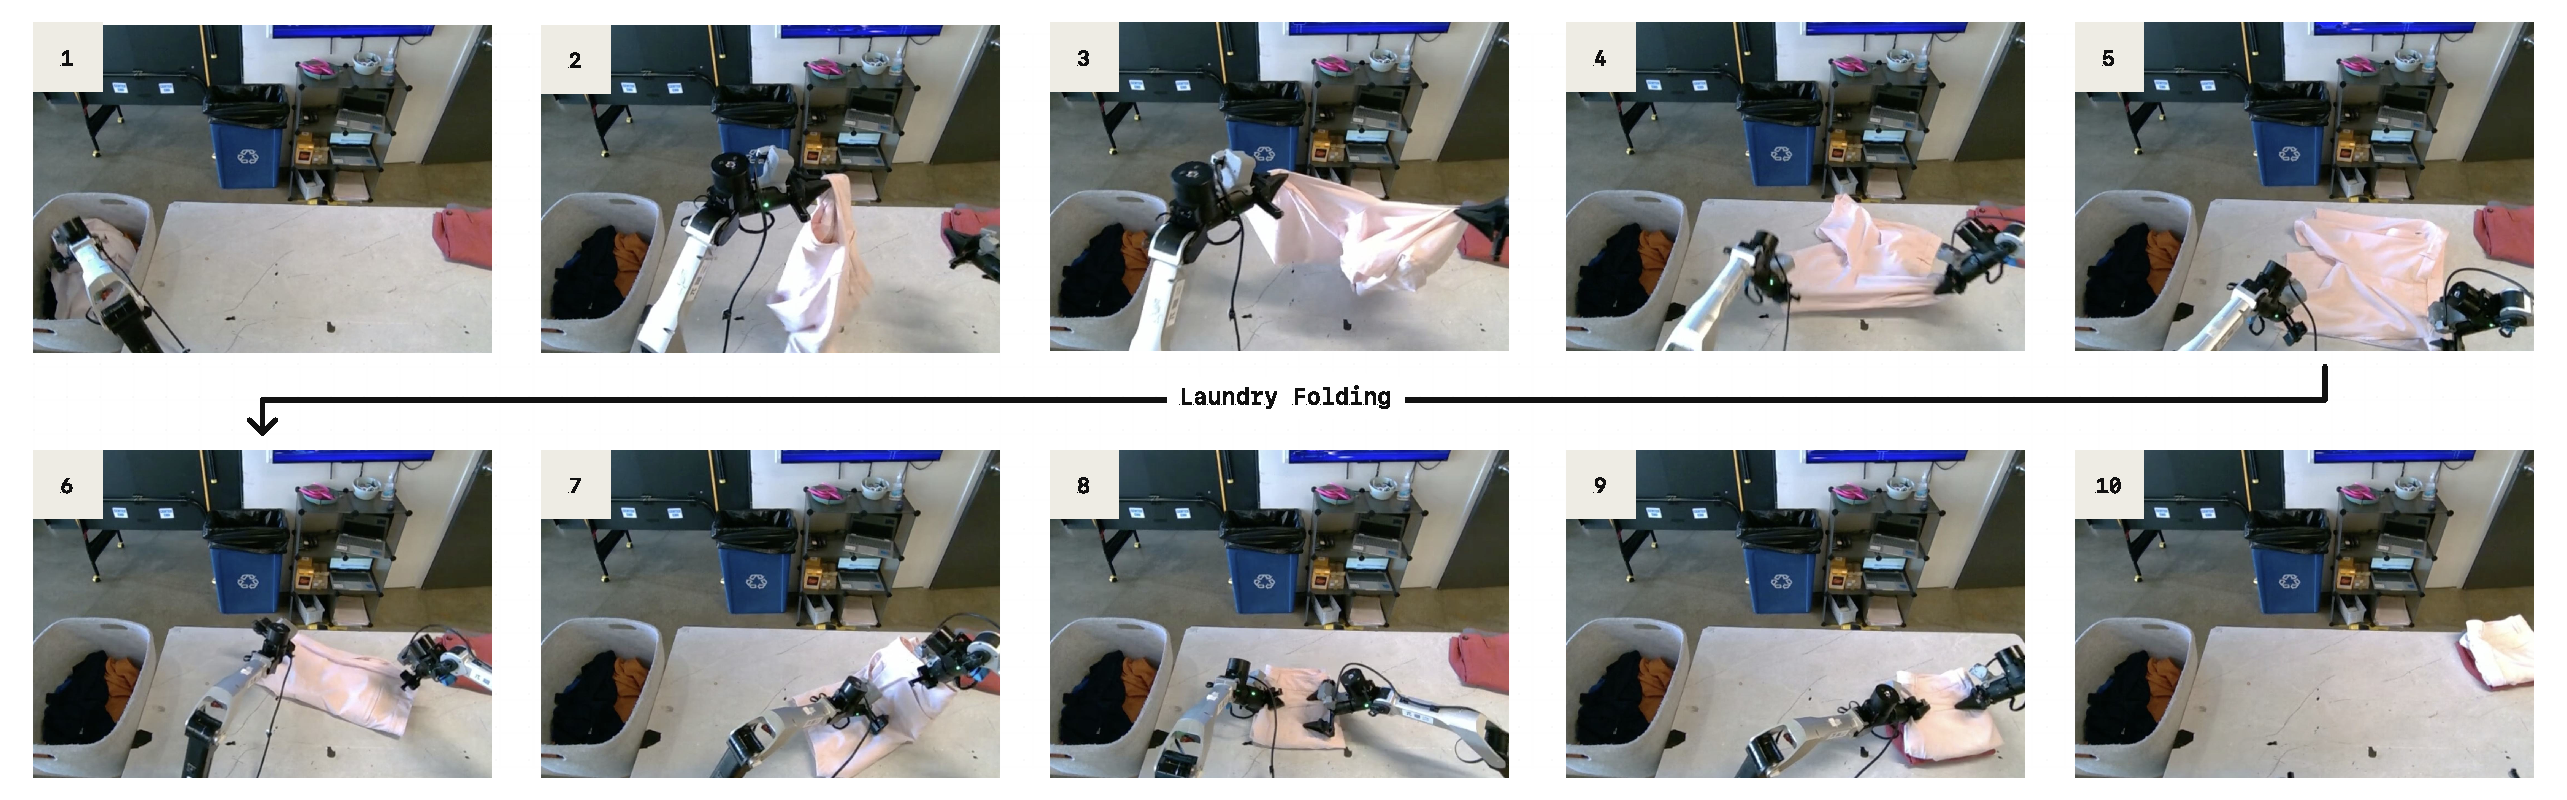
\includegraphics[width=\linewidth]{figures/quali_rollout.pdf}
    \caption{\textbf{Rollout of \GeneralistModelAcronym{} on the laundry folding task.} \ModelAcronym{} tokenization enables autoregressive VLAs to perform complex, long-horizon, and dexterous tasks that were impossible with previous tokenization schemes.
    }
    \label{fig:quali_rollout}
\end{figure*}

One current limitation of the autoregressive VLA is its inference speed: while $\pi_0$ with diffusion typically predicts one second action chunks within 100ms on an NVIDIA 4090 GPU, the $\pi_0$ model with \ModelAcronym{} tokenization needs approximately 750ms of inference time per chunk, since it must perform more autoregressive decoding steps (typically 30-60 action tokens need to be decoded, vs. 10 diffusion steps for diffusion $\pi_0$) and use the full 2B parameter language model backbone for autoregressive decoding (vs. a 300M parameter ``action expert'' for diffusion $\pi_0$). While we did not find this slower inference to hurt performance on the static manipulation tasks we evaluated, it made evaluations significantly slower. Going forward, there are many techniques for accelerating the inference of discrete, autoregressive transformer models that are used extensively in the LLM literature (e.g., speculative decoding, quantization, custom inference kernels, etc.), but we will leave an investigation of these to future work.




\subsection{Scaling Autoregressive VLAs to Large Robot Datasets}
\label{sec:generalist_vlas}

We have demonstrated \ModelAcronym's effectiveness for training autoregressive VLAs on individual robot datasets, but does it scale to training dexterous \emph{generalist} policies? To test this, we train the \GeneralistModelAcronym{} model from the previous section on the cross-embodied robot data mixture used by $\pi_0$~\citep{black2024pi_0}, the largest dexterous robot manipulation dataset to date. It includes 903M timesteps from our own datasets.
Additionally, 9.1\% of the training mixture consists of the open-source datasets BRIDGE v2 \cite{walke2023bridgedata}, DROID \cite{khazatsky2024droid}, and OXE \cite{open_x_embodiment_rt_x_2023}.

\begin{figure}[t]
    \centering
    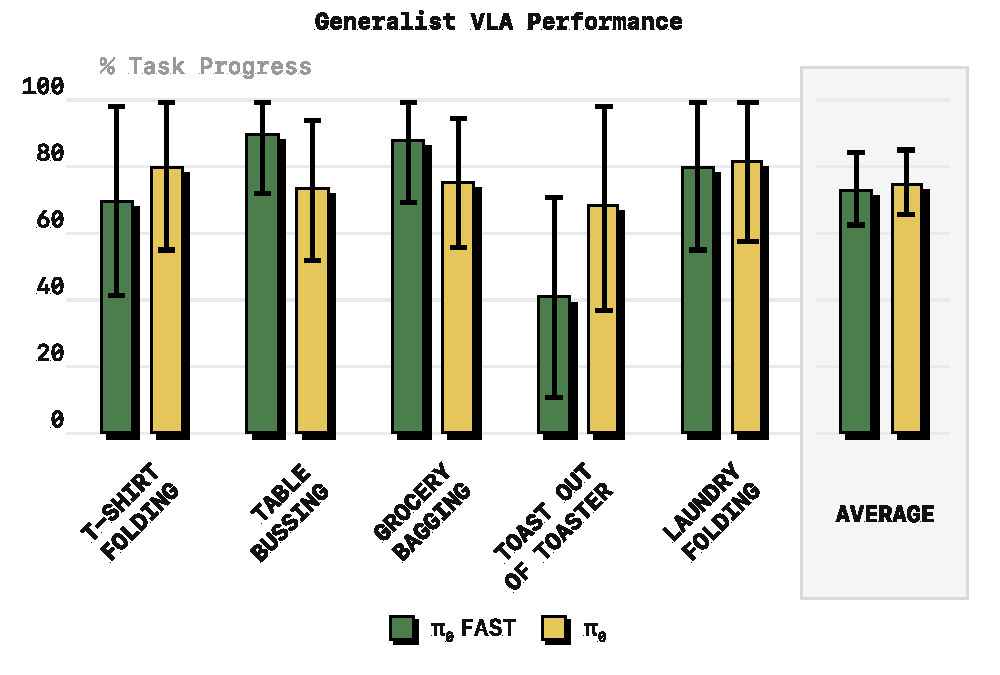
\includegraphics[width=\linewidth]{figures/pi0_multi_task.pdf}
    \caption{\textbf{Comparison of {\GeneralistModelAcronym} and diffusion $\pi_0$~\citep{black2024pi_0} generalist policies.} \GeneralistModelAcronym{} matches the performance of diffusion $\pi_0$ while requiring significantly less compute for training. Reported: mean and 95\% CI.
    }
    \label{fig:pi0_multi_task_comparison}
\end{figure}
We compare zero-shot performance to the diffusion $\pi_0$ model on the tasks from \citet{black2024pi_0} in \cref{fig:pi0_multi_task_comparison}. Overall, we find that the autoregressive \GeneralistModelAcronym{} model matches the performance of the diffusion $\pi_0$ model, including on the most challenging \textit{laundry folding} task, \textbf{while requiring significantly less compute for training}. We show a qualitative example of \GeneralistModelAcronym{} performing the laundry folding task in \cref{fig:quali_rollout} and include additional videos on our website. 

Importantly, we find that \GeneralistModelAcronym{} converges significantly faster than the diffusion $\pi_0$ model: the model in the evaluations above required 5x fewer GPU hours for training than the $\pi_0$ model from \citet{black2024pi_0}. We show robot evaluation results for multiple checkpoints throughout the course of training in \cref{fig:convergence} (averaging performance on two representative tasks: table bussing and t-shirt folding). The results show clearly that \GeneralistModelAcronym{} achieves high performance significantly faster. For state-of-the-art VLA training runs, which can often use thousands of GPU hours, a 5x reduction in required compute is significant. We include a full comparison across all tasks for a compute-matched $\pi_0$ checkpoint in Appendix, \cref{fig:pi0_compute_matched} and find that the same conclusions hold: \GeneralistModelAcronym{} clearly outperforms compute matched $\pi_0$ due to its faster convergence.

To summarize, we have demonstrated that \ModelAcronym{} tokenization allows us to train autoregressive VLAs on complex, dexterous robot tasks that prior tokenization schemes completely fail on. We have also shown that \ModelAcronym{}, when combined with state-of-the-art VLAs like $\pi_0$, scales to training generalist, cross-embodied policies that rival the performance of the best diffusion VLAs while being significantly faster to train. 



